\section{Разработка пользовательского интерфейса} \label{interface}

\subsection{Разработка средств интеграции с текстовыми процессорами} \label{text_processors}

Техническое задание на проект не требует создания полноценного пользовательского интерфейса.
Однако для создания и обработки документов используются текстовые процессоры, интеграция с которыми существенно расширяет поле применения системы электронного документооборота.
Ниже рассмотрены наиболее полпулярные системы обработки документов.

\begin{itemize}[label=\textbf{---} ]
	
	\item \textbf{Простые текстовые редакторы}

	Для создания технической документации часто используется TeX --- компилируемый язык разметки. Для работы с ним достаточно простых текстовых редакторов, обладающих минимальным набором функций (без поддержки форматирования, стилей и т.п.) -- таких, как Vi и Notepad. Режим их работы можно назвать консольным, поэтому для интеграции с ними не требуется графических средств: взаимодействие осуществляется через командный интерфейс.
	
	\item \textbf{Microsoft Office}

	Редакторы семейства Microsoft Office (Word, Excel) используются для создания и форматирования документов в формате docx/xlsx. Несмотря на то, что работа с такими документами также возможна в командном режиме, для полноценной работы с историей необходимо графическое средство сравнения версий документа. MS Office имеет встроенные средства сравнения, однако они рассчитаны на работу с двумя разными файлами, а не с версиями одного файла, хранящегося в структуре системы электронного документооборота. Поэтому было разработано программное обеспечение для взаимодействия СЭД с Microsoft Office. Пример сравнения документов представлен на рис. \ref{img:mso_compare}.
	\begin{figure}[h!]
		\centering
		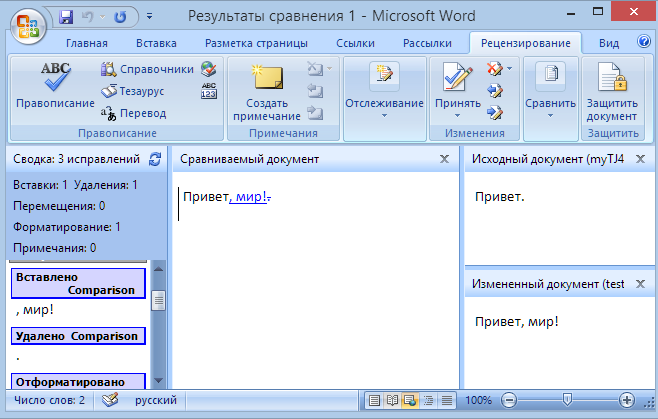
\includegraphics[width=0.85\textwidth]{mso_compare}
		\caption{Сравнение версий документа в Microsoft Word}
		\label{img:mso_compare}
	\end{figure}

	\item \textbf{LibreOffice}

	Для редактирования документов в форматах odt/docx и ods/xlsx используются программы свободного пакета LibreOffice. Это самый распространённый пакет обработки документов в среде Linux. Он так же, как и Microsoft Office, имеет встроенные средства сравнения документов. Для интеграции их с системой электронного документооборота было разработано соответствующее программное обеспечение. Пример сравнения документов представлен на рис. \ref{img:lo_compare}.
	\begin{figure}[h!]
		\centering
		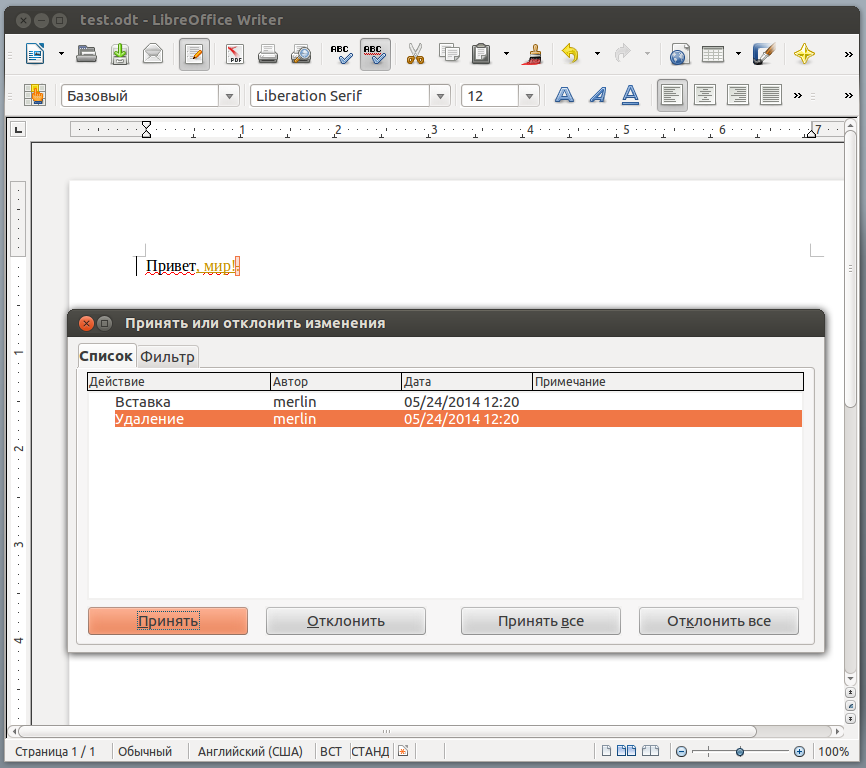
\includegraphics[width=0.85\textwidth]{lo_compare}
		\caption{Сравнение версий документа в LibreOffice Writer}
		\label{img:lo_compare}
	\end{figure}
\end{itemize}
\FloatBarrier

\subsection{Разработка средств просмотра истории документов} \label{git_history}

Для просмотра истории документов был разработан web-интерфейс с индикацией состояния электронной подписи для записей. На рис. \ref{img:good_signature} и \ref{img:bad_signature} показаны случаи корректной и некорректной подписи.

\begin{figure}[h!]
	\centering
	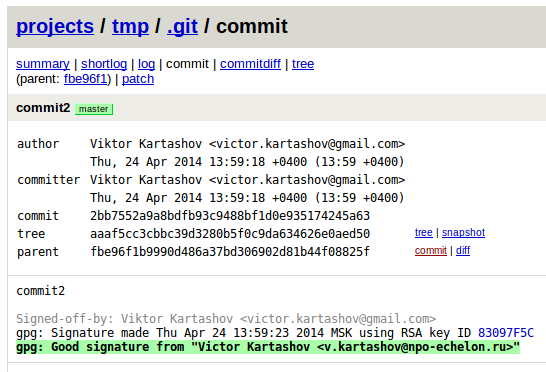
\includegraphics[width=0.7\textwidth]{good_signature}
	\caption{Пример успешной проверки подписи к записи в истории изменений}
	\label{img:good_signature}
\end{figure}

\begin{figure}[h!]
	\centering
	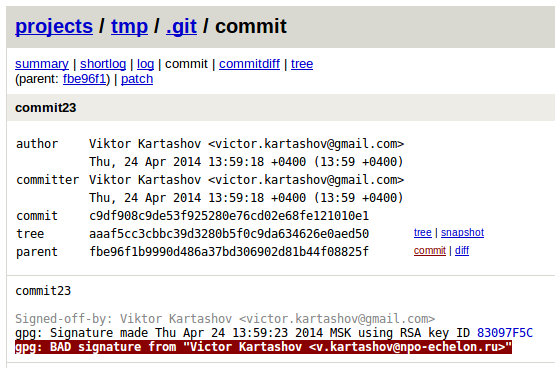
\includegraphics[width=0.7\textwidth]{bad_signature}
	\caption{Пример неуспешной проверки подписи к записи в истории изменений}
	\label{img:bad_signature}
\end{figure}
\FloatBarrier